\chapter{Multi-Party Computation}

\section{Introduction}
Multi-Party Computation (MPC), also known as Secure Function Evaluation, allows two or more parties
to correctly compute a function of their private inputs without exposure, i.e., without
the input of one party being revealed to the other parties.
A generic function \textit{f} receives as input a set $A = \{a_1,a_2,\dots,a_n\}$
of arguments, where $a_i$ is the input of the i-th party, and $1\leq i\leq n$, and outputs a value \textit{z}, which represents the result
of the joint computation of \textit{f}, as shown in Figure \ref{fig:mpcscheme}.
The output of \textit{f} is given by the following expression,
\begin{equation}\label{eq:mpc}
z = f(a_1,a_2,\dots,a_n)
\end{equation}

\renewcommand{\figurename}{Figure}
\begin{figure}[H]
\centering
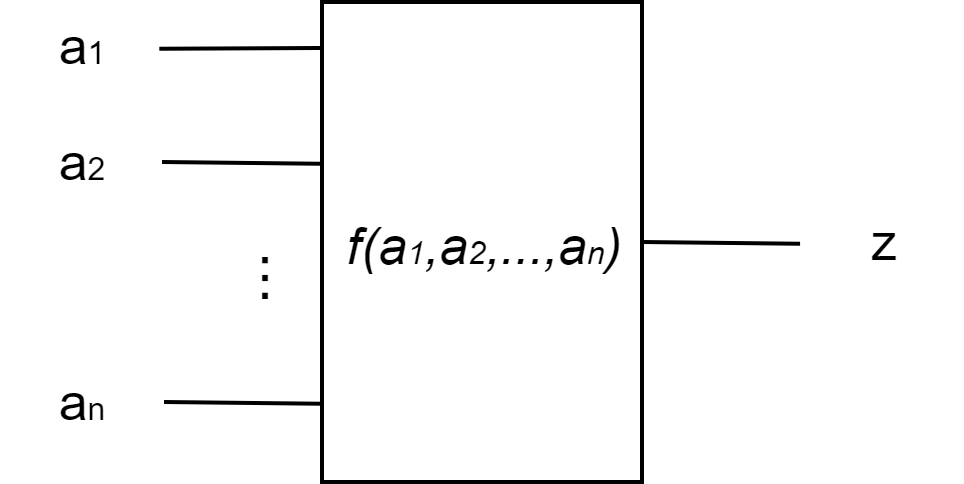
\includegraphics[width=.45\linewidth]{./figures/mpc/mpc_scheme}
\caption{Multi-Party Computation Diagram}
\label{fig:mpcscheme}
\end{figure}
\pagebreak

\section{Two-Party Computation}
Two-Party Computation (2PC) is a specific case of MPC, where a generic function \textit{f} receives as input a set $\{a,b\}$
of arguments, where \textit{a} is the input from the first party and \textit{b} is the input from the second,
and outputs a value \textit{c}, as shown in Figure \ref{fig:tpcscheme}.
The output of \textit{f} is given by the following expression,
\begin{equation}\label{eq:tpc}
c = f(a,b)
\end{equation}

\renewcommand{\figurename}{Figure}
\begin{figure}[H]
\centering
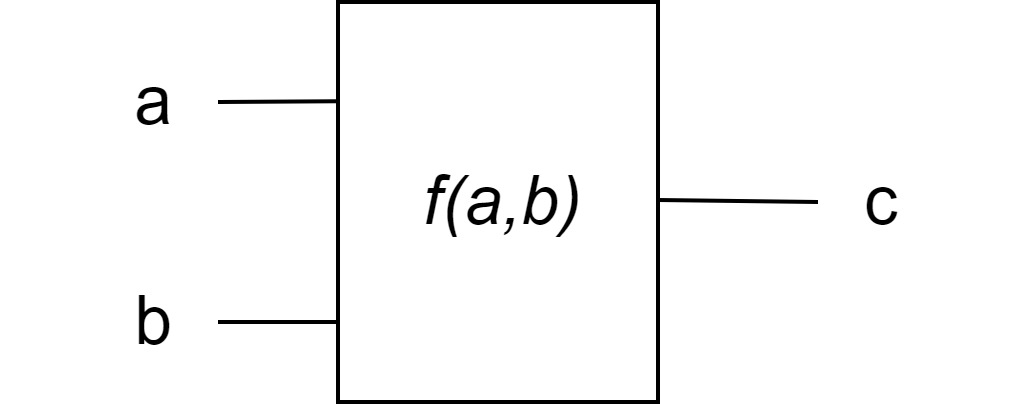
\includegraphics[width=.4\linewidth]{./figures/mpc/two_party_computation_scheme}
\caption{Two-Party Computation Diagram}
\label{fig:tpcscheme}
\end{figure}

\section{Known Problems}
\subsection{Message Access}
Consider 2 parties, Alice and Bob. Alice has a set of messages $A=\{m_0,m_1,m_2,\ldots,m_{n-1}\}$
and Bob has an index $b$. The output of this function should be $m_b$, i.e., the message from Alice's set of index $b$. Bob should not gain
any more information other than $m_b$ and Alice should not know the value of $b$.
\begin{equation}\label{eq:messageaccess}
f(A,b) = A[b]
\end{equation}

\subsection{The Millionaire' Problem}
Consider 2 parties, Alice and Bob, with inputs $a$ and $b$ respectively. The output of this function is $1$ when $a < b$ 
and $0$ when $a $\geq b$. In other terms,
\begin{equation}\label{eq:tpc}
f(a,b) = max(a,b)
\end{equation}

\subsection{Average Value}
Consider 2 parties, Alice and Bob, with inputs $a$ and $b$ respectively. The output of this function should be the average value of $a$ and $b$
. In other terms,
\begin{equation}\label{eq:tpc}
f(a,b) = \frac{a+b}{2}
\end{equation}

\section{Solutions}
In this section we will be presenting the classic solutions to the 3 previous problems. We will later present our approach.
\subsection{With a Third Trusted Party}
For this case we assume that the computation of the function is done by a Trusted Third Party (TTP). 
We will also assume an ideal scenario, where the TTP is not corrupted.
Alice and Bob do not have access to the computation of the function.


\subsubsection{Message Access}
For this example, we will assume that $A = \{1101,0011\}$ and $b = 1$.
\begin{enumerate}
\item Alice and Bob send their inputs, $A$ and $b$ respectively, to the TTP
\item The TTP computes the function and determines $A[1]$
\item The TTP sends $0011$ to Alice and Bob
\end{enumerate}

\subsubsection{The Millionaire' Problem}
For this example, we will assume that $a = 1101$ and $b = 1100$.
\begin{enumerate}
\item Alice and Bob send their inputs, $a$ and $b$ respectively, to the TTP
\item The TTP computes the function and determines $a < b$
\item The TTP sends $0$ to Alice and Bob
\end{enumerate}

\subsubsection{Average Value}
For this example, we will assume that $a = 0100$ and $b = 0010$.
\begin{enumerate}
\item Alice and Bob send their inputs, $a$ and $b$ respectively, to the TTP
\item The TTP computes the function and determines $\frac{a+b}{2}$
\item The TTP sends $0011$ to Alice and Bob
\end{enumerate}

\subsection{One Party Computes the Function}
For this case we consider only 2 parties (a TTP is not necessary) and we assume that the computation is done by one party.
The other party does not have access to the computation.

\subsubsection{Message Access}
%Complete this section
\subsubsection{The Millionaire' Problem}
%Complete this section
\subsubsection{Average Value}
%Complete this section

\subsection{Both Parties Compute the Function}
For this example we consider 2 parties, Alice and Bob. These parties will perform a joint computation of the function, without revealing
their inputs. They have access to their part of the computation.

\subsubsection{Message Access}
Let's consider 2 parties, Alice and Bob. Alice has a set $M = \{m_0,m_1\}$ of messages and Bob has the index, $i$, of the message he wants to receive from Alice, $m_i$.\\
For this example we will be assuming that $i=1$ and $M = \{11,10\}$. Both messages are 2-bit binary numbers.
\begin{enumerate}
%%%%%%%%%%%%%%%%%%%%%%%%%%%%%%%%%%%%%%%%%%%%%%%%%%%%%%%%%%%%%%%%%%%%%%%%%%%%%%%%%%%%%%%%%%%%%%%%%%%%%%%%%%%%%%%%%%%%%%%%
\item Bob generates a 4-bit key, $K_b=0111$ where only the bits of indexes $2i$ and $2i+1$ are known ($C$) to him. Since i=1, Bob only knows the last 2 bits of $K_b$. The remaining 2 bits of $K_b$ are random ($R$), thus unknown to Bob.
\renewcommand{\figurename}{Figure}
\begin{figure}[H]
\centering
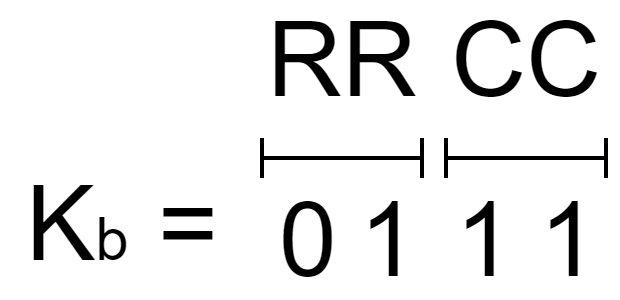
\includegraphics[width=.25\linewidth]{./figures/mpc/mpc_bob_key}
\caption{Known ($C$) and Unknown ($R$) bits from Bob's perspective }
\label{fig:knownbob}
\end{figure}
%%%%%%%%%%%%%%%%%%%%%%%%%%%%%%%%%%%%%%%%%%%%%%%%%%%%%%%%%%%%%%%%%%%%%%%%%%%%%%%%%%%%%%%%%%%%%%%%%%%%%%%%%%%%%%%%%%%%%%%%
\item Bob sends to Alice the set $I = \{2,3\}$ corresponding to the indexes of the bits known to him.
%%%%%%%%%%%%%%%%%%%%%%%%%%%%%%%%%%%%%%%%%%%%%%%%%%%%%%%%%%%%%%%%%%%%%%%%%%%%%%%%%%%%%%%%%%%%%%%%%%%%%%%%%%%%%%%%%%%%%%%%
\item Alice generates a 4-bit key, $K_a=1011$ where the last 2 bits of $K_a$ must be the same as the last 2 of $K_b$. All 4 bits from the key
are unknown to Alice. She doesn't know which 2 bits from $K_a$ are equal to $K_b$ (only Bob has that information),i.e., from her perspective
all bits are random.
\renewcommand{\figurename}{Figure}
\begin{figure}[H]
\centering
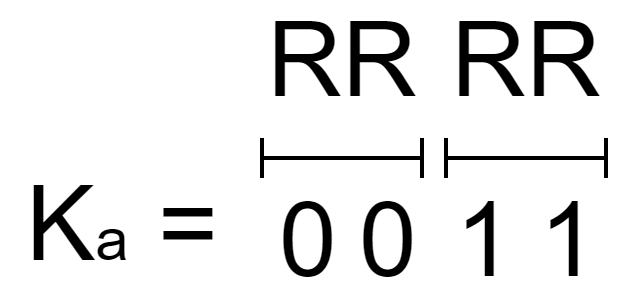
\includegraphics[width=.25\linewidth]{./figures/mpc/mpc_alice_key}
\caption{Known ($C$) and Unknown ($R$) bits from Alice's perspective }
\label{fig:knownalice}
\end{figure}
%%%%%%%%%%%%%%%%%%%%%%%%%%%%%%%%%%%%%%%%%%%%%%%%%%%%%%%%%%%%%%%%%%%%%%%%%%%%%%%%%%%%%%%%%%%%%%%%%%%%%%%%%%%%%%%%%%%%%%%%
\item Alice encrypts the messages with $K_a$ and sends the encrypted information to Bob. In this example, $1101$ will be sent to Bob.
\renewcommand{\figurename}{Figure}
\begin{figure}[H]
\centering
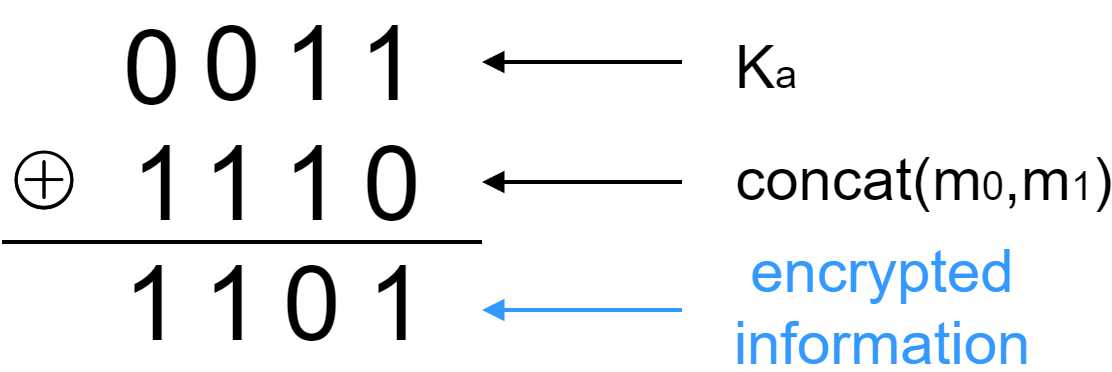
\includegraphics[width=.4\linewidth]{./figures/mpc/mpc_message_encrypting}
\caption{Alice encrypts the messages with $K_a$}
\label{fig:mpcencryption}
\end{figure}
%%%%%%%%%%%%%%%%%%%%%%%%%%%%%%%%%%%%%%%%%%%%%%%%%%%%%%%%%%%%%%%%%%%%%%%%%%%%%%%%%%%%%%%%%%%%%%%%%%%%%%%%%%%%%%%%%%%%%%%%
\item Bob decrypts the information received from Alice with $K_b$ and retrieves the message $m_1$, which correspond to bits of indexes 2 and 3 (since $i=1$).\\
The first two bits of the decrypted information do not represent $m_0$.
\renewcommand{\figurename}{Figure}
\begin{figure}[H]
\centering
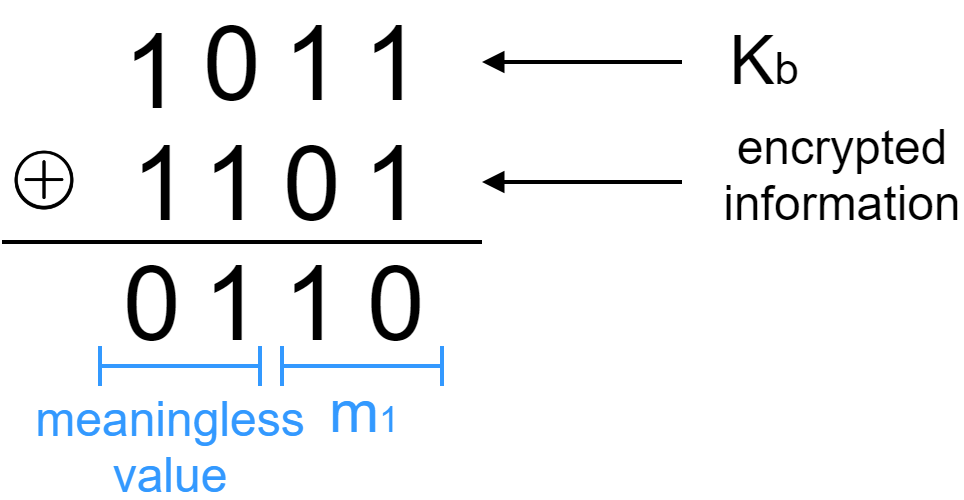
\includegraphics[width=.4\linewidth]{./figures/mpc/mpc_message_decrypting}
\caption{Bob decrypts the information with $K_b$}
\label{fig:mpcdecryption}
\end{figure}
\end{enumerate}

\subsubsection{The Millionaire' Problem}
%Complete this section
\subsubsection{Average Value}
%Complete this section

\section{Oblivious Transfer}
Oblivious Transfer (OT) is a protocol that allows the sender to transfer one piece of information
to a receiver, but remains oblivious as to what piece has been transferred.\\
For example, consider two parties, Alice and Bob, where Alice has a set $M = \{m_0,m_1\}$ of messages
and Bob wants to obtain one of those messages, but won't reveal which one. By OT, Bob is able to
receive the message he wanted from Alice without Alice knowing which one she sent to Bob.

\renewcommand{\figurename}{Figure}
\begin{figure}[H]
\centering
\includegraphics[width=.4\linewidth]{./figures/mpc/OT}
\caption{Oblivious Transfer Diagram}
\label{fig:otscheme}
\end{figure}

\section{Garbled Circuit Protocol}
Introduced in 1986 by Andrew Yao, the Garbled Circuit protocol (GC) addresses the case
of Two-Party Computation (2PC), without the presence of a trusted third party.\\
GC allows a secure evaluation of a function given as a Boolean circuit that is represented as a series of logic gates.
The circuit is known to both parties.\\

\section{Hardware Description Languages}
Contrary to Programming Languages such as C or C++, which are used to specify a set of instructions to a computer, Hardware Description Languages (HDL) are computer languages used to describe the structure and behavior of digital logic circuits. They allow for the synthesis of HDL description code into a netlist (specification of physical eletronic components, such as AND gates or NOT gates, and how they are connected together).

\section{TinyGarble}
TinyGarble is a GC framework that takes advantage of powerful logic synthesis techniques, provided by both HDL synthesis tools
and TinyGarble's custom libraries, in order improve the overall efficiency of the GC protocol.\\
It it possible to describe the circuit using High-Level Programming Languages (HLPL) such as C, although High-Level Synthesis (HLS) is required. HLS is performed by High-Level Synthesis tools, such as SPARK for the C language.

\renewcommand{\figurename}{Figure}
\begin{figure}[H]
\centering
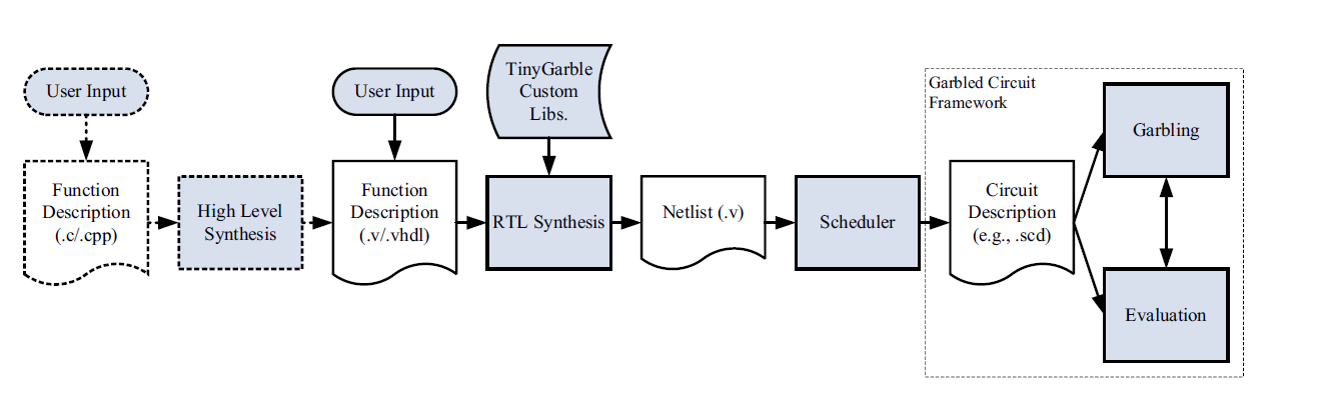
\includegraphics[width=.9\linewidth]{./figures/mpc/tinygarble_flow_diagram}
\caption{TinyGarble Flow Diagram}
\label{fig:tgdiagram}
\end{figure}

\section{ARM2GC}
Although circuit description in HLPL is possible, it is not very efficient when compared to HDL circuit description. ARM2GC addresses this problem, significantly improving the performance of garbled circuits described in HLPL.\\
In the case of 2PC, ARM2GC's approach to GC is based on the ARM processor architecture and consists in providing a public parameter to function \textit{f}, so that its output would be given by the following expression,
\begin{equation}\label{eq:arm2gc}
z = f(a,b,p)
\end{equation}
, where $p$ represents a public parameter, known to both parties.\\
In ARM2GC the Boolean circuit required to perform GC is that of a processor to which the compiled binary of the function is given as a public input ($p$\textit{ = compiled binary of the function}). This optimization is performed by the SkipGate algorithm.

\bibliography{./chapter/mpcomputation} 